% How primes p < 240 factor in Z[sqrt(-5)] (generated; see Chapter 11).
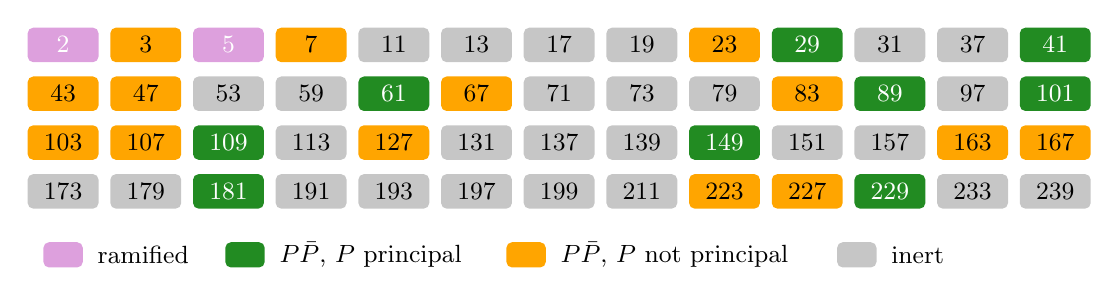
\begin{tikzpicture}[x=1.05cm,y=0.62cm]
  \node[fill=Plum,text=white,rounded corners=2pt,minimum width=0.9cm,font=\small] at (0,0) {2};
  \node[fill=Orange,text=black,rounded corners=2pt,minimum width=0.9cm,font=\small] at (1,0) {3};
  \node[fill=Plum,text=white,rounded corners=2pt,minimum width=0.9cm,font=\small] at (2,0) {5};
  \node[fill=Orange,text=black,rounded corners=2pt,minimum width=0.9cm,font=\small] at (3,0) {7};
  \node[fill=gray!45,text=black,rounded corners=2pt,minimum width=0.9cm,font=\small] at (4,0) {11};
  \node[fill=gray!45,text=black,rounded corners=2pt,minimum width=0.9cm,font=\small] at (5,0) {13};
  \node[fill=gray!45,text=black,rounded corners=2pt,minimum width=0.9cm,font=\small] at (6,0) {17};
  \node[fill=gray!45,text=black,rounded corners=2pt,minimum width=0.9cm,font=\small] at (7,0) {19};
  \node[fill=Orange,text=black,rounded corners=2pt,minimum width=0.9cm,font=\small] at (8,0) {23};
  \node[fill=ForestGreen,text=white,rounded corners=2pt,minimum width=0.9cm,font=\small] at (9,0) {29};
  \node[fill=gray!45,text=black,rounded corners=2pt,minimum width=0.9cm,font=\small] at (10,0) {31};
  \node[fill=gray!45,text=black,rounded corners=2pt,minimum width=0.9cm,font=\small] at (11,0) {37};
  \node[fill=ForestGreen,text=white,rounded corners=2pt,minimum width=0.9cm,font=\small] at (12,0) {41};
  \node[fill=Orange,text=black,rounded corners=2pt,minimum width=0.9cm,font=\small] at (0,-1) {43};
  \node[fill=Orange,text=black,rounded corners=2pt,minimum width=0.9cm,font=\small] at (1,-1) {47};
  \node[fill=gray!45,text=black,rounded corners=2pt,minimum width=0.9cm,font=\small] at (2,-1) {53};
  \node[fill=gray!45,text=black,rounded corners=2pt,minimum width=0.9cm,font=\small] at (3,-1) {59};
  \node[fill=ForestGreen,text=white,rounded corners=2pt,minimum width=0.9cm,font=\small] at (4,-1) {61};
  \node[fill=Orange,text=black,rounded corners=2pt,minimum width=0.9cm,font=\small] at (5,-1) {67};
  \node[fill=gray!45,text=black,rounded corners=2pt,minimum width=0.9cm,font=\small] at (6,-1) {71};
  \node[fill=gray!45,text=black,rounded corners=2pt,minimum width=0.9cm,font=\small] at (7,-1) {73};
  \node[fill=gray!45,text=black,rounded corners=2pt,minimum width=0.9cm,font=\small] at (8,-1) {79};
  \node[fill=Orange,text=black,rounded corners=2pt,minimum width=0.9cm,font=\small] at (9,-1) {83};
  \node[fill=ForestGreen,text=white,rounded corners=2pt,minimum width=0.9cm,font=\small] at (10,-1) {89};
  \node[fill=gray!45,text=black,rounded corners=2pt,minimum width=0.9cm,font=\small] at (11,-1) {97};
  \node[fill=ForestGreen,text=white,rounded corners=2pt,minimum width=0.9cm,font=\small] at (12,-1) {101};
  \node[fill=Orange,text=black,rounded corners=2pt,minimum width=0.9cm,font=\small] at (0,-2) {103};
  \node[fill=Orange,text=black,rounded corners=2pt,minimum width=0.9cm,font=\small] at (1,-2) {107};
  \node[fill=ForestGreen,text=white,rounded corners=2pt,minimum width=0.9cm,font=\small] at (2,-2) {109};
  \node[fill=gray!45,text=black,rounded corners=2pt,minimum width=0.9cm,font=\small] at (3,-2) {113};
  \node[fill=Orange,text=black,rounded corners=2pt,minimum width=0.9cm,font=\small] at (4,-2) {127};
  \node[fill=gray!45,text=black,rounded corners=2pt,minimum width=0.9cm,font=\small] at (5,-2) {131};
  \node[fill=gray!45,text=black,rounded corners=2pt,minimum width=0.9cm,font=\small] at (6,-2) {137};
  \node[fill=gray!45,text=black,rounded corners=2pt,minimum width=0.9cm,font=\small] at (7,-2) {139};
  \node[fill=ForestGreen,text=white,rounded corners=2pt,minimum width=0.9cm,font=\small] at (8,-2) {149};
  \node[fill=gray!45,text=black,rounded corners=2pt,minimum width=0.9cm,font=\small] at (9,-2) {151};
  \node[fill=gray!45,text=black,rounded corners=2pt,minimum width=0.9cm,font=\small] at (10,-2) {157};
  \node[fill=Orange,text=black,rounded corners=2pt,minimum width=0.9cm,font=\small] at (11,-2) {163};
  \node[fill=Orange,text=black,rounded corners=2pt,minimum width=0.9cm,font=\small] at (12,-2) {167};
  \node[fill=gray!45,text=black,rounded corners=2pt,minimum width=0.9cm,font=\small] at (0,-3) {173};
  \node[fill=gray!45,text=black,rounded corners=2pt,minimum width=0.9cm,font=\small] at (1,-3) {179};
  \node[fill=ForestGreen,text=white,rounded corners=2pt,minimum width=0.9cm,font=\small] at (2,-3) {181};
  \node[fill=gray!45,text=black,rounded corners=2pt,minimum width=0.9cm,font=\small] at (3,-3) {191};
  \node[fill=gray!45,text=black,rounded corners=2pt,minimum width=0.9cm,font=\small] at (4,-3) {193};
  \node[fill=gray!45,text=black,rounded corners=2pt,minimum width=0.9cm,font=\small] at (5,-3) {197};
  \node[fill=gray!45,text=black,rounded corners=2pt,minimum width=0.9cm,font=\small] at (6,-3) {199};
  \node[fill=gray!45,text=black,rounded corners=2pt,minimum width=0.9cm,font=\small] at (7,-3) {211};
  \node[fill=Orange,text=black,rounded corners=2pt,minimum width=0.9cm,font=\small] at (8,-3) {223};
  \node[fill=Orange,text=black,rounded corners=2pt,minimum width=0.9cm,font=\small] at (9,-3) {227};
  \node[fill=ForestGreen,text=white,rounded corners=2pt,minimum width=0.9cm,font=\small] at (10,-3) {229};
  \node[fill=gray!45,text=black,rounded corners=2pt,minimum width=0.9cm,font=\small] at (11,-3) {233};
  \node[fill=gray!45,text=black,rounded corners=2pt,minimum width=0.9cm,font=\small] at (12,-3) {239};
  \begin{scope}[shift={(0,-4.3)},font=\small]
    \node[fill=Plum,minimum width=0.5cm,minimum height=0.32cm,rounded corners=2pt] at (0.0,0) {}; \node[right] at (0.3,0) {ramified};
    \node[fill=ForestGreen,minimum width=0.5cm,minimum height=0.32cm,rounded corners=2pt] at (2.2,0) {}; \node[right] at (2.5,0) {$P\bar P$, $P$ principal};
    \node[fill=Orange,minimum width=0.5cm,minimum height=0.32cm,rounded corners=2pt] at (5.6,0) {}; \node[right] at (5.9,0) {$P\bar P$, $P$ not principal};
    \node[fill=gray!45,minimum width=0.5cm,minimum height=0.32cm,rounded corners=2pt] at (9.6,0) {}; \node[right] at (9.9,0) {inert};
  \end{scope}
\end{tikzpicture}
